\section{Analisi statica CheckStyle}

\subsection{Introduzione}

Garantire la qualità del codice sorgente è fondamentale per assicurare la stabilità, l'affidabilità e la manutenibilità delle applicazioni. Tra gli strumenti utilizzati per questo scopo, l'analisi statica del codice riveste un ruolo cruciale. In questo Progetto è quindi stato utilizzato \textbf{Checkstyle}, \href{https://checkstyle.sourceforge.io/}{https://checkstyle.sourceforge.io/}, che permette una valutazione automatica della conformità del codice e linee guida da seguire.
\\
Questo documento si propone di fornire una panoramica dettagliata sull'utilizzo di Checkstyle per condurre analisi statiche del codice sorgente. Esploreremo le sue funzionalità, le principali regole di analisi implementate e i benefici derivanti dall'integrazione di questa pratica nella fase di sviluppo del software. Vengono ora mostrati alcuni report generati dai vari microservizi.


È inoltre possibile visualizzare per intero i report generati nei seguenti documenti:


\begin{itemize}
	\item Gestione Comanda: 
	
	{\small 	\href{https://giorgio-hash.github.io/ServeEasy/Report/GestioneComanda/site/checkstyle.html}{https://giorgio-hash.github.io/ServeEasy/Report/GestioneComanda/site/checkstyle.html}}
	\item Gestione Cliente: 
	
	{\small 	\href{https://giorgio-hash.github.io/ServeEasy/Report/GestioneCliente/site/checkstyle.html}{https://giorgio-hash.github.io/ServeEasy/Report/GestioneCliente/site/checkstyle.html}}
	\item Gestione Cucina: 
	
	{\small \href{https://giorgio-hash.github.io/ServeEasy/Report/GestioneCucina/site/checkstyle.html}{https://giorgio-hash.github.io/ServeEasy/Report/GestioneCucina/site/checkstyle.html}}
\end{itemize}
Per poter visualizzare i file di report online si è utilizzato il servizio offerto da GitHub: GitHub Pages\cite{github-pages}, esso permette di ospitare siti web statici generati da repository GitHub pubbliche.

\newpage

\subsection{Report Gestione Comanda}

\begin{figure}[htbp]
	\centering
	\includegraphics[scale=0.6]{iterazione1/images/Cs_Summary_Gestione_Comanda.jpg}
	\caption{Sommario di gestione comanda\label{fig:Cs_Summary_Gestione_Comanda}}
\end{figure}

\begin{figure}[htbp]
	\centering
	\includegraphics[scale=0.8]{iterazione1/images/Cs_rules_Gestione_Comanda.jpg}
	\caption{Rules generate da gestione comanda\label{fig:Cs_Rules_Gestione_Comanda}}
\end{figure}

\begin{figure}[H]
	\centering
	\begin{minipage}[b]{1\textwidth}
		\centering
		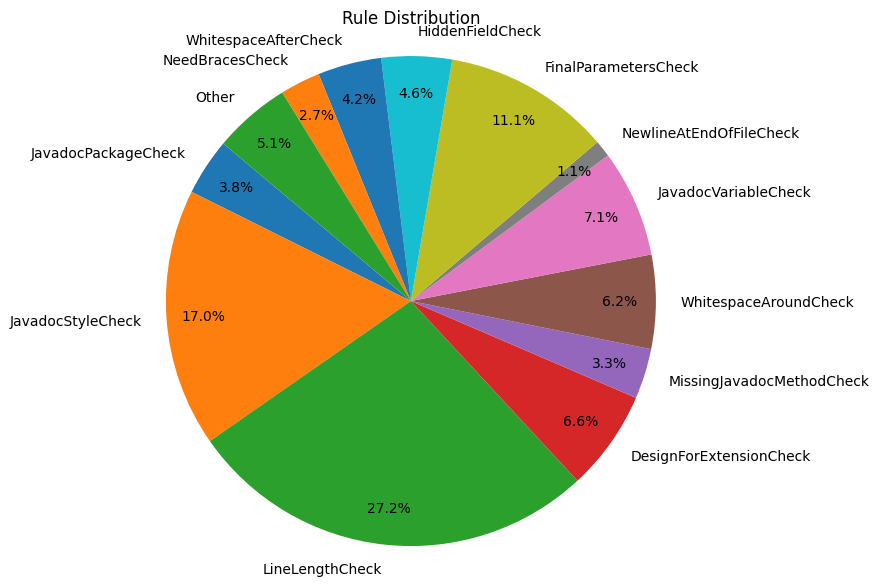
\includegraphics[width=\textwidth]{iterazione1/images/comanda-error_distribution_pie_chart.png}
		\caption{Grafico di tutte le regole}
		\label{fig:comanda-error_distribution_pie_chart}
	\end{minipage}
	\hfill
	\begin{minipage}[b]{0.45\textwidth}
		\centering
		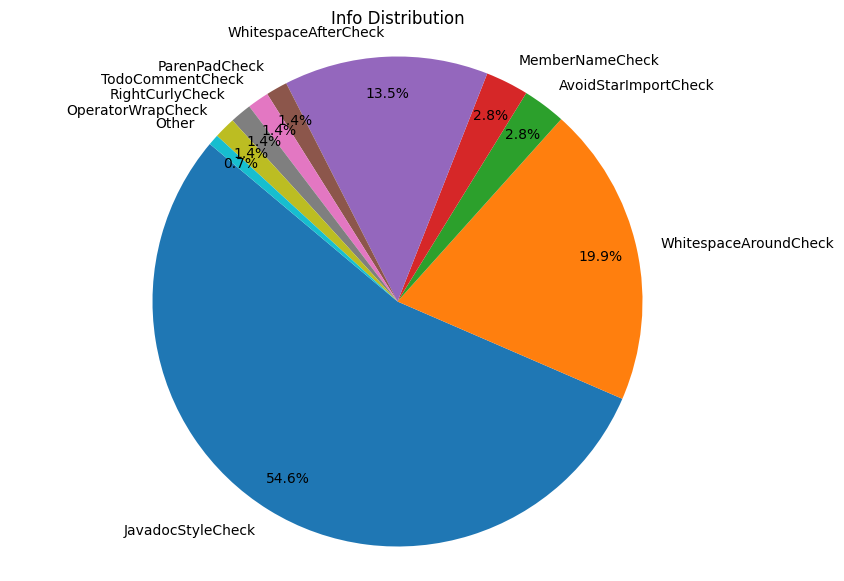
\includegraphics[width=\textwidth]{iterazione1/images/comanda-info_severity_distribution_pie_chart.png}
		\caption{Grafico delle info}
		\label{fig:comanda-info_severity_distribution_pie_chart}
	\end{minipage}
	\vspace{0.5cm}
	\begin{minipage}[b]{0.45\textwidth}
		\centering
		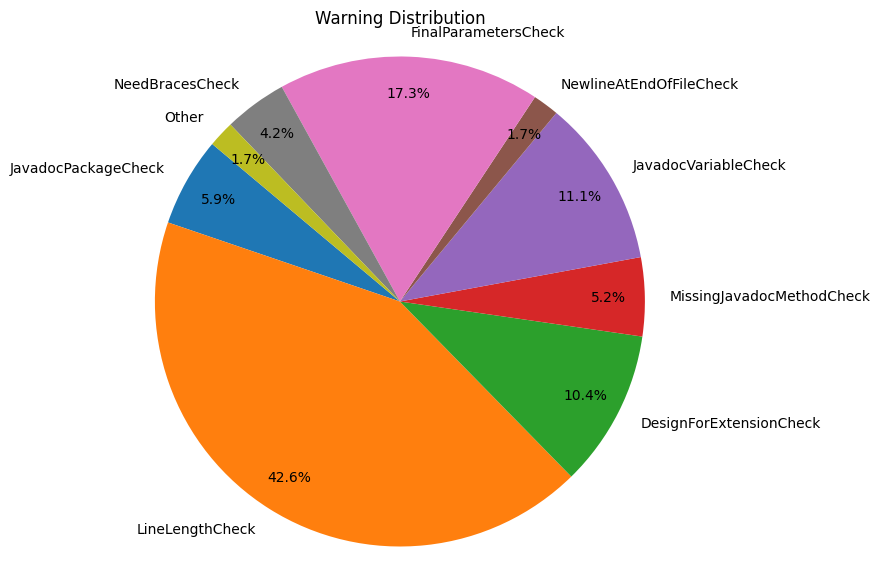
\includegraphics[width=\textwidth]{iterazione1/images/comanda-warning_severity_distribution_pie_chart.png}
		\caption{Grafico degli warnings}
		\label{fig:comanda-warning_severity_distribution_pie_chart}
	\end{minipage}
	\hfill
	\begin{minipage}[b]{0.45\textwidth}
		\centering
		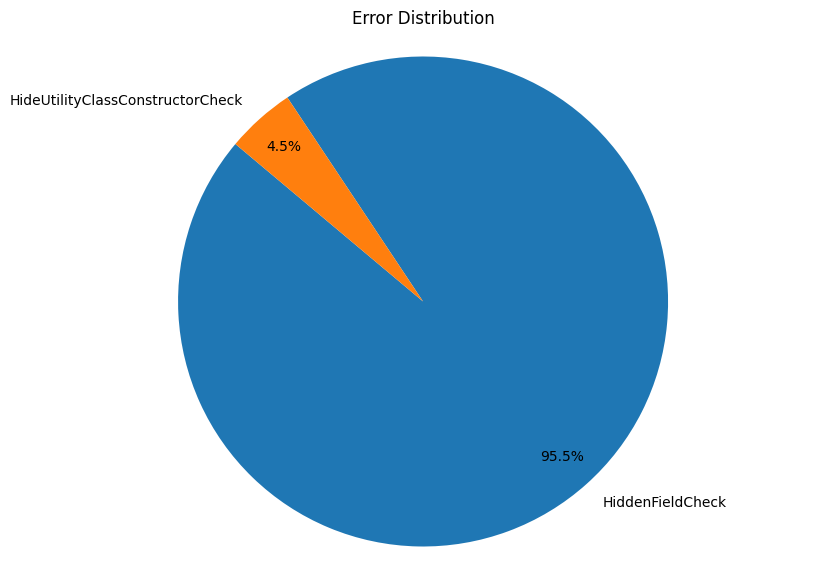
\includegraphics[width=\textwidth]{iterazione1/images/comanda-error_severity_distribution_pie_chart.png}
		\caption{Grafico degli errori}
		\label{fig:comanda-error_severity_distribution_pie_chart}
	\end{minipage}
\end{figure}

\newpage

\subsection{Report Gestione Cliente}

\begin{figure}[htbp]
	\centering
	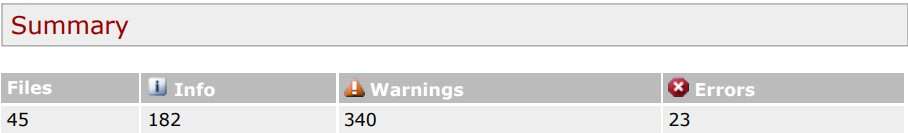
\includegraphics[scale=0.6]{iterazione1/images/Cs_Summary_Gestione_Cliente.jpg}
	\caption{Sommario di gestione cliente\label{fig:Cs_Summary_Gestione_Cliente}}
\end{figure}

\begin{figure}[htbp]
	\centering
	\includegraphics[scale=0.8]{iterazione1/images/Cs_rules_Gestione_Cliente.jpg}
	\caption{Rules generate da gestione cliente\label{fig:Cs_Rules_Gestione_Cliente}}
\end{figure}

\begin{figure}[H]
	\centering
	\begin{minipage}[b]{1\textwidth}
		\centering
		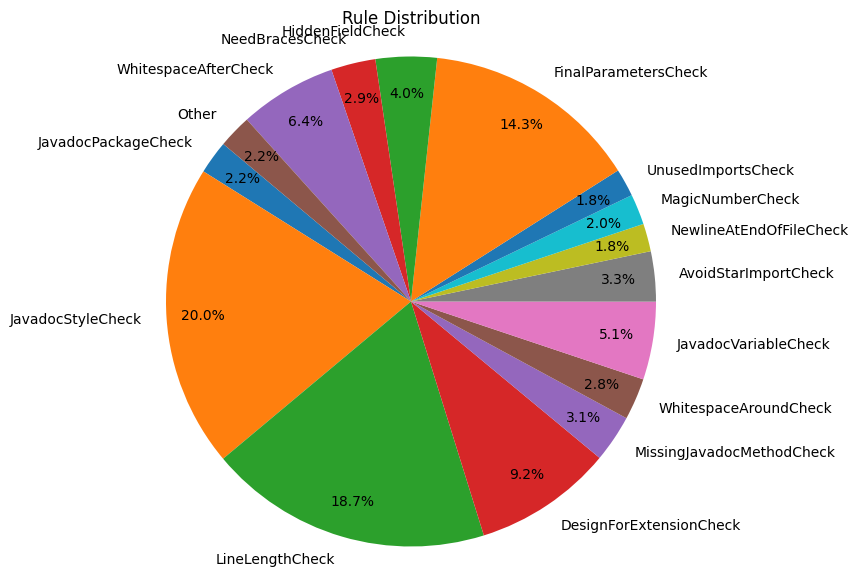
\includegraphics[width=\textwidth]{iterazione1/images/cliente-error_distribution_pie_chart.png}
		\caption{Grafico di tutte le regole}
		\label{fig:cliente-error_distribution_pie_chart}
	\end{minipage}
	\hfill
	\begin{minipage}[b]{0.45\textwidth}
		\centering
		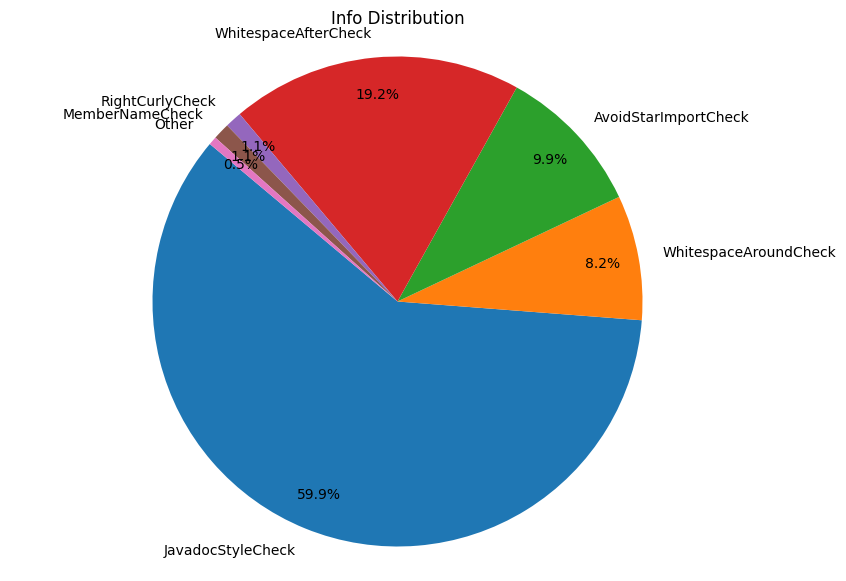
\includegraphics[width=\textwidth]{iterazione1/images/cliente-info_severity_distribution_pie_chart.png}
		\caption{Grafico delle info}
		\label{fig:cliente-info_severity_distribution_pie_chart}
	\end{minipage}
	\vspace{0.5cm}
	\begin{minipage}[b]{0.45\textwidth}
		\centering
		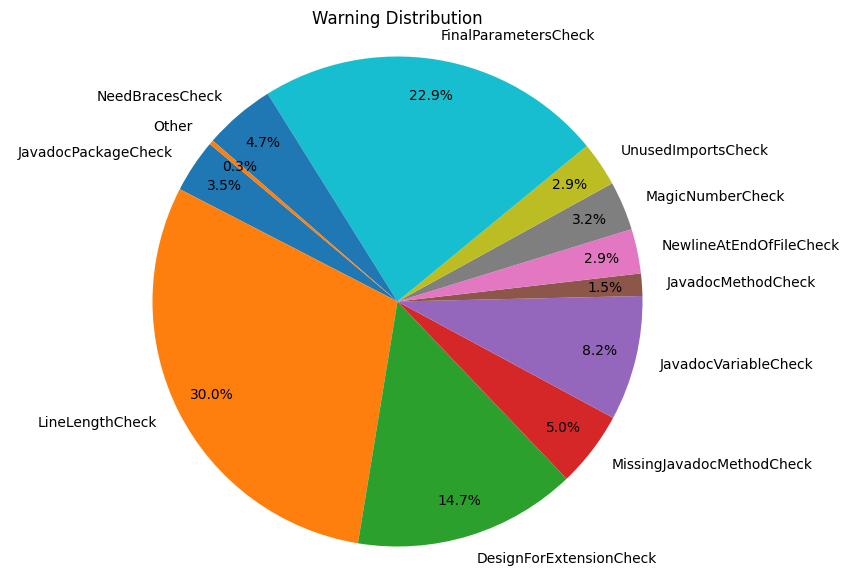
\includegraphics[width=\textwidth]{iterazione1/images/cliente-warning_severity_distribution_pie_chart.png}
		\caption{Grafico degli warnings}
		\label{fig:cliente-warning_severity_distribution_pie_chart}
	\end{minipage}
	\hfill
	\begin{minipage}[b]{0.45\textwidth}
		\centering
		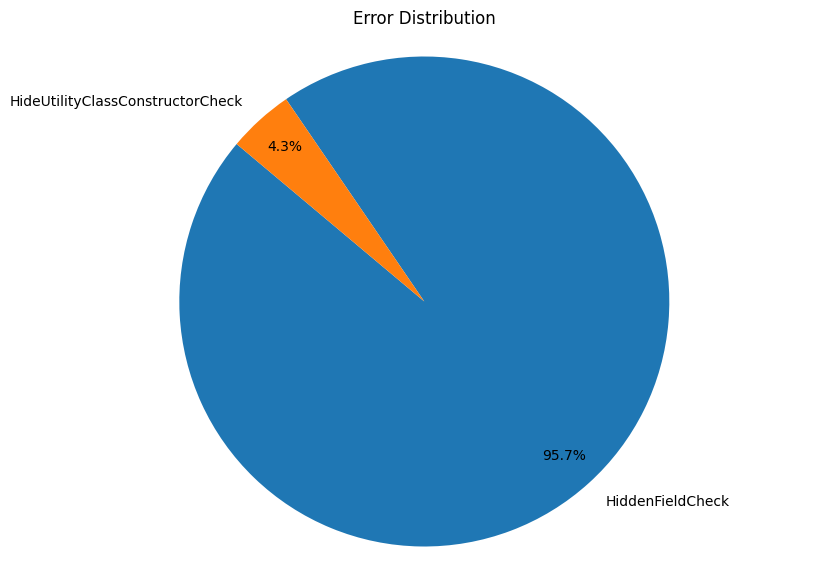
\includegraphics[width=\textwidth]{iterazione1/images/cliente-error_severity_distribution_pie_chart.png}
		\caption{Grafico degli errori}
		\label{fig:cliente-error_severity_distribution_pie_chart}
	\end{minipage}
\end{figure}

\newpage

\subsection{Report Gestione Cucina}

\begin{figure}[htbp]
	\centering
	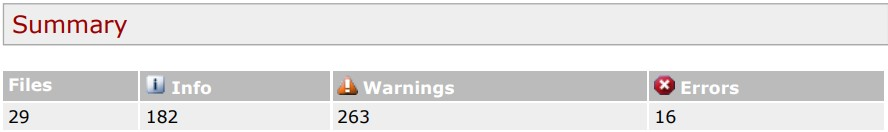
\includegraphics[scale=0.6]{iterazione1/images/Cs_Summary_Gestione_Cucina.jpg}
	\caption{Sommario di gestione cucina\label{fig:Cs_Summary_Gestione_Cucina}}
\end{figure}

\begin{figure}[htbp]
	\centering
	\includegraphics[scale=0.9]{iterazione1/images/Cs_rules_Gestione_Cucina.jpg}
	\caption{Rules generate da gestione cucina\label{fig:Cs_Rules_Gestione_Cucina}}
\end{figure}

\begin{figure}[H]
	\centering
	\begin{minipage}[b]{1\textwidth}
		\centering
		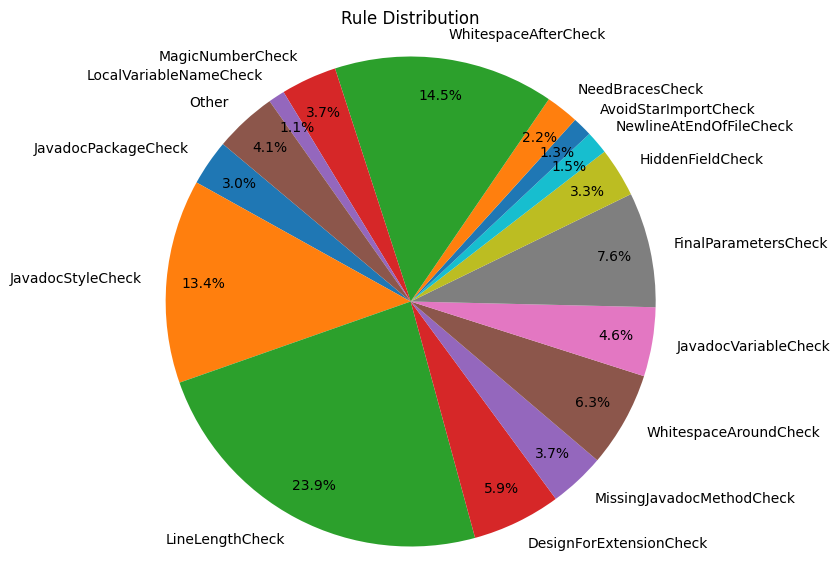
\includegraphics[width=\textwidth]{iterazione1/images/cucina-error_distribution_pie_chart.png}
		\caption{Grafico di tutte le regole}
		\label{fig:cucina-error_distribution_pie_chart}
	\end{minipage}
	\hfill
	\begin{minipage}[b]{0.45\textwidth}
		\centering
		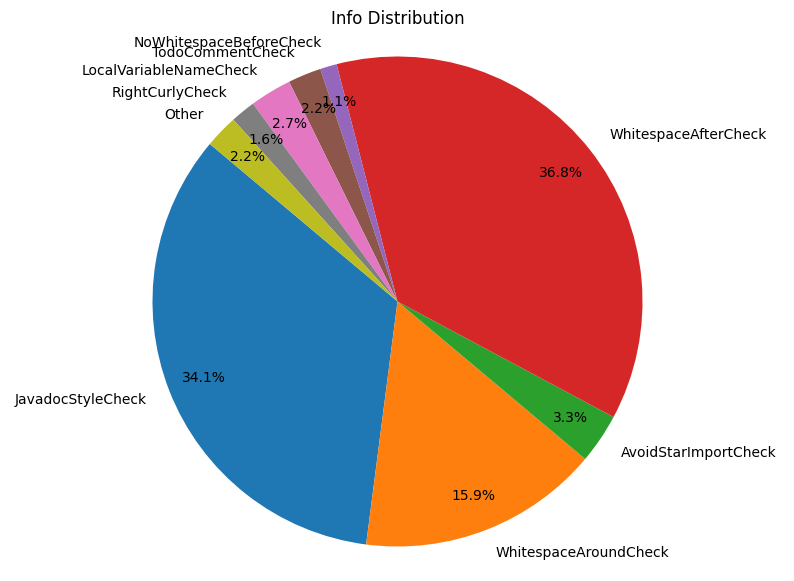
\includegraphics[width=\textwidth]{iterazione1/images/cucina-info_severity_distribution_pie_chart.png}
		\caption{Grafico delle info}
		\label{fig:cucina-info_severity_distribution_pie_chart}
	\end{minipage}
	\vspace{0.5cm}
	\begin{minipage}[b]{0.45\textwidth}
		\centering
		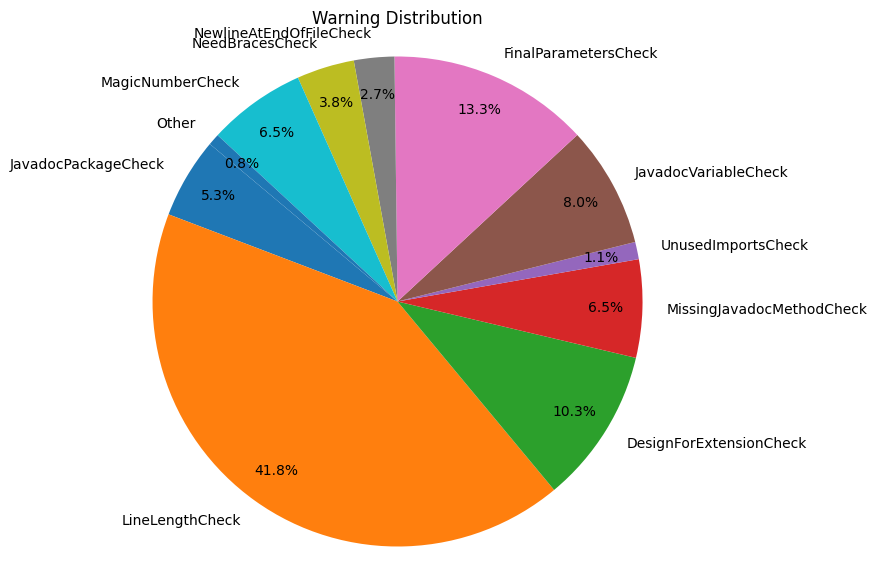
\includegraphics[width=\textwidth]{iterazione1/images/cucina-warning_severity_distribution_pie_chart.png}
		\caption{Grafico degli warnings}
		\label{fig:cucina-warning_severity_distribution_pie_chart}
	\end{minipage}
	\hfill
	\begin{minipage}[b]{0.45\textwidth}
		\centering
		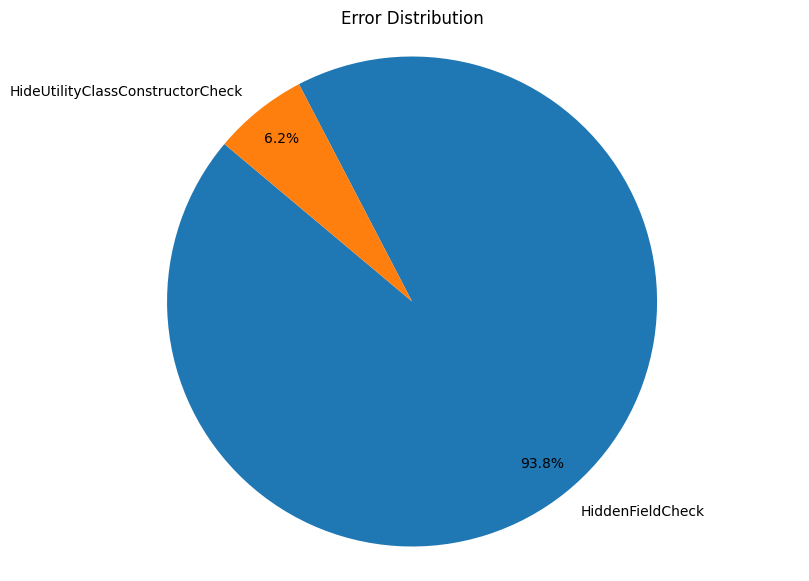
\includegraphics[width=\textwidth]{iterazione1/images/cucina-error_severity_distribution_pie_chart.png}
		\caption{Grafico degli errori}
		\label{fig:cucina-error_severity_distribution_pie_chart}
	\end{minipage}
\end{figure}


\newpage

\subsection{Specifica}
Di seguito vengono ora date le Specifiche segnalate dai vari report.

\paragraph{Errors:}

	\begin{itemize}

		\item La regola \textbf{\textbf{HiddenField}} controlla se una variabile locale o un parametro ha lo stesso nome di un campo \text{(field)} definito nella stessa classe.

		\item La regola \textbf{\textbf{hideUtilityClassConstructor}} si assicura che le classi di tilità non abbiano un costruttore pubblico. Le classi di utilità sono spesso utilizzate per raggruppare funzionalità comuni e non dovrebbero essereistanziate direttamente. Pertanto, i costruttori di queste classi dovrebbero essere privati o, se si desidera consentire l’ereditarietà, protetti.

	\end{itemize}

\paragraph{Warning:}

	\begin{itemize}

		\item La regola \textbf{\textbf{NeedBraces}} controlla se i blocchi di codice \text{(if, else, for, while, ecc.)} sono racchiusi tra parentesi graffe.

		\item La regola \textbf{\textbf{MagicNumber}} controlla se ci sono numeri letterali nel codice che non sono definiti come costanti. In altre parole, i“magic numbers” sono valori numerici che compaiono direttamente nel codice senza essere assegnati a una variabile o costante.

		\item La regola \textbf{\textbf{designForExtension}} controlla se le classi sono progettate per essere estese tramite sottoclassi. È particolarmente utile nei progetti di librerie (non nei progetti di applicazioni) che si preoccupano di seguire un design OOP ideale per garantire che le classi funzionino correttamente in tutti i casi, anche in caso di uso improprio.

		\item La regola \textbf{\textbf{UnusedImports}} verifica gli import nonutilizzati all’interno del codice.

		\item La regola \textbf{\textbf{JavadocMethod}} controlla la documentazione Javadoc di un metodo o di un costruttore.

		\item La regola \textbf{\textbf{JavadocPackage}} verifica che ogni pacchetto Javaabbia un file Javadoc utilizzato per i commenti. Di default, consente solo un file package-info.java, ma può essere configurata per consentire un file “package.html” Verrà segnalata una violazione se entrambi i file esistono,poiché ciò non è consentito dallo strumento Javadoc.

		\item La regola \textbf{\textbf{JavadocVariable}} controlla se una variabile ha uncommento Javadoc. Viene segnalata una violazione se manca il commento Javadoc per qualsiasi membro di visibilità.

		\item La regola \textbf{\textbf{MissingJavadocMethod}} verifica la presenza di commenti Javadoc mancanti per metodi o costruttori.

		\item La regola \textbf{\textbf{FinalParameters}} verifica che i parametri per metodi, costruttori, blocchi catch e blocchi for-each siano dichiarati come final. Tuttavia, i metodi di interfaccia, astratti e nativi non vengono controllati: la parola chiave final non ha senso per i parametri dei metodi di interfaccia, astratti e nativi poiché non esiste alcun codice che potrebbe modificare il parametro.

		\item La regola \textbf{\textbf{NewlineAtEndOfFile}} verifica se i file terminano con un separatore di riga.

		\item La regola \textbf{\textbf{LineLength verifica}} se le righe sono troppo lunghe. Questo è importante perché le righe lunghe possono essere difficili da leggere,specialmente quando si stampa il codice o quando gli sviluppatori hanno uno spazio limitato sullo schermo (ad esempio, se l’IDE mostra altre informazioni come l’albero del progetto o la gerarchia delle classi).

	\end{itemize}

\paragraph{Info:}

	\begin{itemize}

		\item La regola \textbf{\textbf{LeftCurly}} controlla la posizione delle parentesi graffe aperte all’interno dei blocchi di codice.

		\item La regola \textbf{\textbf{RightCurly}} controlla se le parentesi graffe chiuse sono posizionate correttamente all’interno dei blocchi di codice.

		\item La regola \textbf{\textbf{AvoidStarImport}} controlla se ci sono dichiarazioni di importazione che utilizzano l’asterisco *. Importare tutte le classi da un pacchetto o membri statici da una classe porta a un accoppiamento stretto tra pacchetti o classi e potrebbe causare problemi quando una nuovaversione di una libreria introduce conflitti di nomi.

		\item La regola \textbf{\textbf{JavadocStyle}} verifica che i commenti Javadoc siano ben formati. (punteggiatura alla fine della prima frase, verifica della presenza di descrizione, verifica dei tag html incompleti, verifica documentazione del pacchetto, tag html consentiti).

		\item La regola \textbf{\textbf{TodoComment}} verifica la presenza di commenti con la parola chiave “TODO:”. In realtà, è un matcher generico di pattern per i commenti Java. Per verificare altri pattern nei commenti Java, è possibile impostare la proprietà format. L’utilizzo dei commenti “TODO:” è un ottimo modo per tenere traccia dei compiti da svolgere.

		\item La regola \textbf{\textbf{LocalVariableName}} verifica che i nomi delle variabili locali (variabili dichiarate all’interno di un metodo o di un blocco)siano conformi a un pattern specificato.

		\item La regola \textbf{\textbf{MethodParamPad}} controlla la spaziatura tra l’identificatore di una definizione di metodo, una definizione di costruttore,una chiamata di metodo o una chiamata di costruttore e la parentesi sinistra della lista dei parametri.

		\item La regola \textbf{\textbf{NoWhitespaceBefore}}  verifica che non ci sia spazio bianco prima di un token specifico. In particolare, controlla che il token non sia preceduto da spazio bianco

		\item La regola \textbf{\textbf{OperatorWrap}} verifica come gli operatori sono posizionati rispetto alle righe di codice. In particolare, controlla se gli operatori dovrebbero essere posizionati sulla stessa riga o su una nuova riga. Questo è importante per mantenere la leggibilità del codice e per seguire le convenzioni di stile.

		\item La regola \textbf{\textbf{ParenPad}} verifica come le parentesi sono posizionate rispetto alle righe di codice. In particolare, controlla se le parentesi dovrebbero essere seguite da spazio o se devono essere adiacenti senza spazi.

		\item La regola \textbf{\textbf{WhitespaceAfter}} controlla come gli spazi bianchi sono posizionati rispetto ai token nel codice sorgente. In particolare,verifica se gli operatori dovrebbero essere seguiti da spazio o se devono essere adiacenti senza spazi.

		\item La regola \textbf{\textbf{WhitespaceAround}}  verifica che un token sia circondato da spazio bianco. Questa regola si applica a vari contesti, come loop vuoti e lambda vuote.

		\item La regola \textbf{\textbf{redundantModifier}} è progettata per individuare e segnalare i modificatori ridondanti all'interno del codice sorgente Java. Questa regola controlla i modificatori di accesso, come public, protected,private, e anche i modificatori come final, abstract, static e strictfp.

	\end{itemize}

\subsection{Checkstyle}

\paragraph{Installazione:}
Per poter utilizzare le funzionalità di checkstyle all'interno dell'IDEA itelliJ è stato installa un plugin disponibile all'interno del marketplace di IntelliJ, ovvero CheckStyle-IDEA\cite{jetbrains}. Di seguito viene mostrata la schermata che permette l'installazione di quest'ultima.

\begin{figure}[htbp]
	\centering
	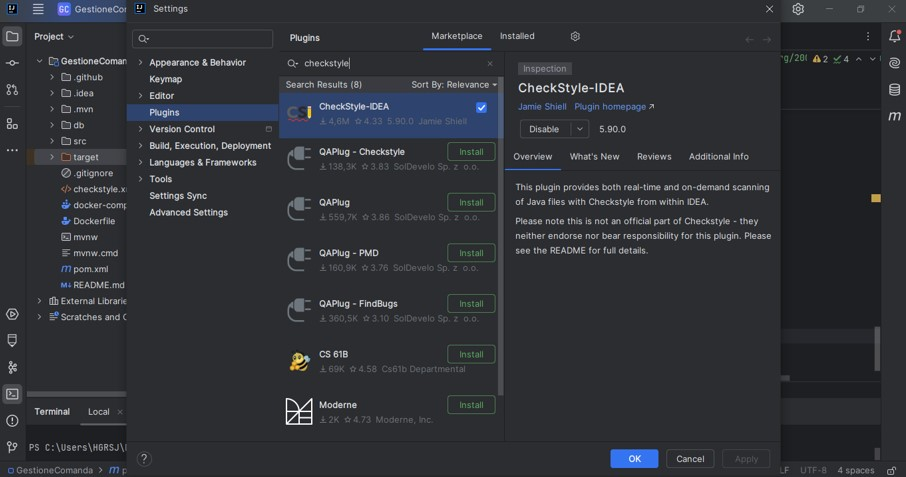
\includegraphics[scale=0.8]{iterazione1/images/Install_checkstyle_intelliJ.jpg}
	\caption{Schermata installazione plugin\label{fig:Install_checkstyle_intelliJ}}
\end{figure}

\paragraph{Configurazione e personalizzazione:}
Per la configurazione del plugin di checkstyle in maven è stato introdotto all'interno del file \textbf{pom.xml} la seguente: 

\begin{lstlisting}[language=XML, caption={plugin Maven con Maven Checkstyle Plugin}]
<plugin>
	<groupId>org.apache.maven.plugins</groupId>
	<artifactId>maven-checkstyle-plugin</artifactId>
	<version>3.3.1</version>
	<configuration>
		<configLocation>checkstyle.xml</configLocation>
	</configuration>
	<executions>
		<execution>
			<goals>
				<goal>checkstyle</goal>
			</goals>
		</execution>
	</executions>
</plugin>
\end{lstlisting}

Abbiamo quindi creato un file Checkstyle.xml personalizzando le regole di Sun Checkstyle, che definiscono un insieme di regole di programmazione per la scrittura del codice. Questo ci aiuta a adattare le regole alle nostre specifiche esigenze, garantendo uno stile di codifica coerente e di alta qualità. Le categorie di violazioni controllate sono: Blocks, coding, design, javadoc, imports, misc, naming, sizes, whitespace e modifier.

\begin{lstlisting}[language=XML, caption={Personalizzazioni regole di Sun Checkstyle}]
<?xml version="1.0"?>
<!DOCTYPE module PUBLIC
        "-//Checkstyle//DTD Checkstyle Configuration 1.3//EN"
        "https://checkstyle.org/dtds/configuration_1_3.dtd">

<!--
  Checkstyle configuration that checks the sun coding
-->

<module name="Checker">

    <property name="severity" value="error"/>

    <property name="fileExtensions" value="java, properties, xml"/>

    <!-- Excludes all 'module-info.java' files              -->
    <module name="BeforeExecutionExclusionFileFilter">
        <property name="fileNamePattern" value="module\-info\.java$"/>
    </module>

    <module name="SuppressionFilter">
        <property name="file" value="${org.checkstyle.sun.suppressionfilter.config}"
                  default="checkstyle-suppressions.xml" />
        <property name="optional" value="true"/>
    </module>

    <!-- Checks that a package-info.java file exists for each package.     -->
    <module name="JavadocPackage">
        <property name="severity" value="warning"/>
    </module>

    <!-- Checks whether files end with a new line.                        -->
    <module name="NewlineAtEndOfFile">
        <property name="severity" value="warning"/>
    </module>

    <!-- Checks that property files contain the same keys.         -->
    <module name="Translation"/>

    <!-- Checks for Size Violations.                    -->
    <module name="FileLength">
        <property name="severity" value="warning"/>
    </module>
    <module name="LineLength">
        <property name="fileExtensions" value="java"/>
        <property name="severity" value="warning"/>
    </module>

    <!-- Checks for whitespace                               -->
    <module name="FileTabCharacter">
        <property name="severity" value="warning"/>
    </module>

    <module name="TreeWalker">

        <!-- Checks for Javadoc comments.                     -->
        <module name="InvalidJavadocPosition">
            <property name="severity" value="warning"/>
        </module>
        <module name="JavadocMethod">
            <property name="severity" value="warning"/>
        </module>
        
        <!-- Checks for Naming Conventions.                  -->
        <module name="ConstantName">
            <property name="severity" value="info"/>
        </module>
        <module name="LocalFinalVariableName">
            <property name="severity" value="info"/>
        
        <!-- Checks for imports                              -->
        <module name="AvoidStarImport">
            <property name="severity" value="info"/>
        </module>
        <module name="IllegalImport"> 

        <!-- Checks for Size Violations.                    -->
        <module name="MethodLength">
            <property name="severity" value="info"/>
        </module>
        <module name="ParameterNumber">
            <property name="severity" value="info"/>
        </module>

        <!-- Checks for whitespace                               -->
        <module name="EmptyForIteratorPad">
            <property name="severity" value="info"/>
        </module>
        <module name="GenericWhitespace">
            <property name="severity" value="info"/>
        </module>

        <!-- Checks for blocks. You know, those {}'s         -->
        <module name="AvoidNestedBlocks">
            <property name="severity" value="warning"/>
        </module>
        <module name="EmptyBlock">
            <property name="severity" value="error"/>
        </module>

        <!-- Checks for class design                         -->
        <module name="DesignForExtension">
            <property name="severity" value="warning"/>
        </module>
        <module name="FinalClass">
            <property name="severity" value="warning"/>
        </module>


        <module name="SuppressionXpathFilter">
            <property name="file" value="${org.checkstyle.sun.suppressionxpathfilter.config}"
                      default="checkstyle-xpath-suppressions.xml" />
            <property name="optional" value="true"/>
        </module>

    </module>

</module>
\end{lstlisting}

\paragraph{Esecuzione:}
Avvenuta la fase di installazione e configurazione è ora possibile identificare e correggere le violazioni di stile definite nel file di configurazione.

Per eseguire il controllo di stile è sufficiente eseguire il comando:
\begin{lstlisting}[style=terminal, 
	caption={Avvio controllo checkstyle}]
mvn site
\end{lstlisting}

Esso permetterà di generare all'interno della directory \textbf{target > site} contenente i file html e xml con i report generati.



\subsection{Generazione Grafi}
Al fine di poter visualizzare con più semplicità i file di report sono stati generati dei grafici a torta che mostrano il tipo di errore rilevato e la percentuale delle volte in cui è stato commesso.
Per creare questi grafici abbiamo creato un semplice script python da allegare al progetto di ogni microservizio. 
\subsubsection{Script Python}
Questo script si basa sul file "checkstyle-result.xml" generato dal report di checkstyle e posizionato nella cartella target, quindi come prima cosa viene caricato questo file:
\begin{lstlisting}[style=pythonstyle, caption={Script Python - aggiunta checkstyle-result.xml}, label=lst:python-checkstyle-result]
script_dir = os.path.dirname(os.path.abspath(__file__))
input_xml_file = 
	os.path.join(script_dir, "target", "checkstyle-result.xml")
\end{lstlisting}
Successivamente si passa a fare il parsing di questo file, andando a scandire i vari elementi <error> per ogni singolo <file>, in particoalre si classificano gli errori in base all'attributo severity che può essere info, warning ed error. In questo modo si creano 3 dizionari con questi tipi di valore di severità, oltre a un altro globale che contiene la somma di tutti e 3 gli errori chiamato rule, ed ad ogni occorrenza di un errore data dall'attributo source di error si aumenta il conteggio del dizionario alla chiave corrispondente a quel attributo. Come mostrato da questo pezzo di codice:
\begin{lstlisting}[style=pythonstyle, caption={Script Python - parsing checkstyle-result.xml}, label=lst:python-parsing]
tree = Et.parse(xml_file)
root = tree.getroot()
error_counts = defaultdict(int)
for file in root.findall('file'):
	for error in file.findall('error'):
		if error.get('severity') == severity or skip is True:
			source = error.get('source')
			error_counts[error_type] += 1
\end{lstlisting}
Successivamente si passa a convertire ogni dizionario in un file csv, il quale sarà costruito in modo tale da avere come prima colonna il tipo di errore e come seconda il numero di volte che è stato commesso quell'errore.
Nel passo successivo questi file csv vengono convertiti in un grafico a torta utilizzando la libreria matplotlib.pyplot e salvati in un file png.
\begin{lstlisting}[style=pythonstyle, caption={Script Python - Plot pie chart}, label=lst:python-piechart]
errors = list(error_counts.keys())
counts = list(error_counts.values())
[...]
plt.figure(figsize=(10, 7))
patches, texts, _ = plt.pie(counts, labels=errors, autopct='%1.1f%%', startangle=140, pctdistance=0.85)
plt.axis('equal')
plt.title(title + " Distribution")
plt.savefig(output_file, bbox_inches='tight')
\end{lstlisting}
I file csv e le immagini png vengono salvati nella cartella di percorso target/output/csv per i primi, mentre target/output/images per le seconde.
\paragraph{Come avviarlo:}
per poter avviare lo script python è necessario avere Python installato sul proprio PC\cite{phoenixnap} ed eseguire il seguente comando per installare le librerie necessarie:
\begin{lstlisting}[style=terminal, 
	caption={Python - installare i pacchetti necessari}, label=lst:python-pip-install]
pip install -r python/requirements.txt
\end{lstlisting}
Successivamente eseguire il seguente per poter avviare lo script:
\begin{lstlisting}[style=terminal, 
	caption={Avvio script python}, label=lst:python-main]
python main.py
\end{lstlisting}
È possibile trovare i file generati in target/output dalla root del progetto.
\paragraph{Output:}
esempio di file csv in output:
\begin{lstlisting}[style=pythonstyle, caption={file checkstyle\_warning\_severity\_counts.csv warning di gestione comanda}, label=lst:csv-warning]
Warning,Count
JavadocPackageCheck,17
LineLengthCheck,123
DesignForExtensionCheck,30
MissingJavadocMethodCheck,15
UnusedImportsCheck,2
JavadocVariableCheck,32
JavadocMethodCheck,2
NewlineAtEndOfFileCheck,5
MagicNumberCheck,1
FinalParametersCheck,50
NeedBracesCheck,12
\end{lstlisting}
Grafico a torta associato:
\begin{figure}[htbp]
	\centering
	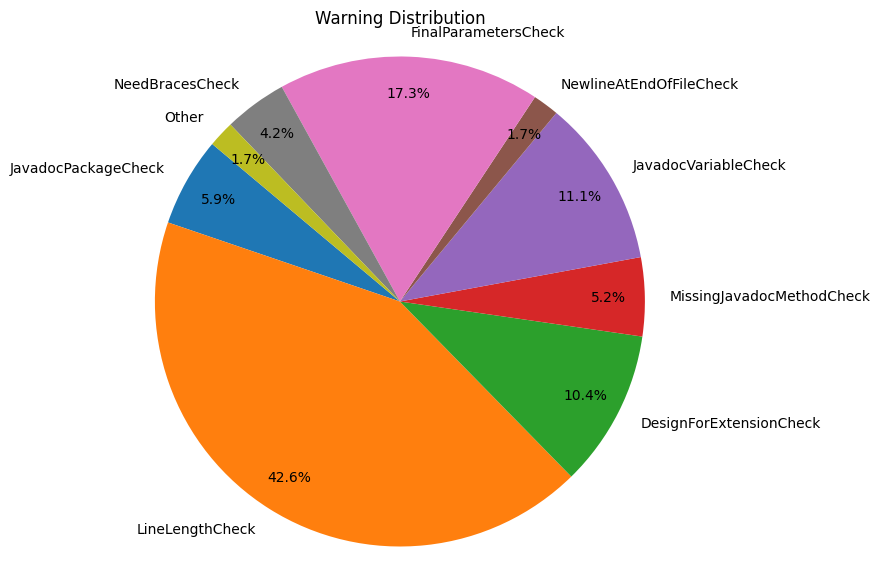
\includegraphics[scale=0.6]{iterazione1/images/warning_severity_distribution_pie_chart.png}
	\caption{Grafico warnings di gestione comanda\label{fig:graph_warning_gestionecomanda}}
\end{figure}

\clearpage